% Options for packages loaded elsewhere
\PassOptionsToPackage{unicode}{hyperref}
\PassOptionsToPackage{hyphens}{url}
%
\documentclass[
]{article}
\usepackage{amsmath,amssymb}
\usepackage{iftex}
\ifPDFTeX
  \usepackage[T1]{fontenc}
  \usepackage[utf8]{inputenc}
  \usepackage{textcomp} % provide euro and other symbols
\else % if luatex or xetex
  \usepackage{unicode-math} % this also loads fontspec
  \defaultfontfeatures{Scale=MatchLowercase}
  \defaultfontfeatures[\rmfamily]{Ligatures=TeX,Scale=1}
\fi
\usepackage{lmodern}
\ifPDFTeX\else
  % xetex/luatex font selection
\fi
% Use upquote if available, for straight quotes in verbatim environments
\IfFileExists{upquote.sty}{\usepackage{upquote}}{}
\IfFileExists{microtype.sty}{% use microtype if available
  \usepackage[]{microtype}
  \UseMicrotypeSet[protrusion]{basicmath} % disable protrusion for tt fonts
}{}
\makeatletter
\@ifundefined{KOMAClassName}{% if non-KOMA class
  \IfFileExists{parskip.sty}{%
    \usepackage{parskip}
  }{% else
    \setlength{\parindent}{0pt}
    \setlength{\parskip}{6pt plus 2pt minus 1pt}}
}{% if KOMA class
  \KOMAoptions{parskip=half}}
\makeatother
\usepackage{xcolor}
\usepackage[margin=1in]{geometry}
\usepackage{graphicx}
\makeatletter
\newsavebox\pandoc@box
\newcommand*\pandocbounded[1]{% scales image to fit in text height/width
  \sbox\pandoc@box{#1}%
  \Gscale@div\@tempa{\textheight}{\dimexpr\ht\pandoc@box+\dp\pandoc@box\relax}%
  \Gscale@div\@tempb{\linewidth}{\wd\pandoc@box}%
  \ifdim\@tempb\p@<\@tempa\p@\let\@tempa\@tempb\fi% select the smaller of both
  \ifdim\@tempa\p@<\p@\scalebox{\@tempa}{\usebox\pandoc@box}%
  \else\usebox{\pandoc@box}%
  \fi%
}
% Set default figure placement to htbp
\def\fps@figure{htbp}
\makeatother
\setlength{\emergencystretch}{3em} % prevent overfull lines
\providecommand{\tightlist}{%
  \setlength{\itemsep}{0pt}\setlength{\parskip}{0pt}}
\setcounter{secnumdepth}{5}
\usepackage{bookmark}
\IfFileExists{xurl.sty}{\usepackage{xurl}}{} % add URL line breaks if available
\urlstyle{same}
\hypersetup{
  pdftitle={Visualizing the Uninsured: A Data Science Perspective on U.S. Health Coverage},
  hidelinks,
  pdfcreator={LaTeX via pandoc}}

\title{Visualizing the Uninsured: A Data Science Perspective on U.S.
Health Coverage}
\author{Eduardo Sáenz-Messía Laborda, 2861597\\
Catherina Mikhail, 2847118\\
Charlotte Craenen, 2865572\\
Hugo van As, 2848225\\
Indy Pleijter, 2810379\\
Julian Zeguers, 2772646\\
Wies Polderman, 2824987\\
Tutorial group 5, group 4 -- J.F. Fitzgerald}
\date{2025-06-24}

\begin{document}
\maketitle

{
\setcounter{tocdepth}{2}
\tableofcontents
}
\subsection{\texorpdfstring{\textbf{Part 1 -- Identify a Social
Problem}}{Part 1 -- Identify a Social Problem}}\label{part-1-identify-a-social-problem}

\subsection{Describe the Social
Problem}\label{describe-the-social-problem}

The substantial number of uninsured people in the United States
represents a significant public health challenge with serious
implications for individuals and the healthcare system. Current data
shows that over 27 million Americans, approximately one in twelve
people, lack health insurance coverage as of 2022 (KFF, 2023). This
coverage gap creates considerable barriers to healthcare access and
produces widespread effects on both individual and population health
outcomes.

For uninsured individuals, the consequences are particularly severe.
Research indicates that people without insurance are significantly more
likely to postpone or forgo necessary medical care due to cost concerns,
leading to poorer health outcomes, increased emergency department
utilization for preventable conditions, and higher mortality rates from
treatable diseases. The economic burden is equally substantial, as
uninsured individuals face full payment responsibility for medical
services, frequently resulting in medical debt, compromised credit
status, and prolonged financial hardship (Davis, 2007).

The impact extends beyond individual consequences to affect the broader
healthcare system. When uninsured patients cannot meet their payment
obligations, healthcare institutions must absorb these costs as
uncompensated care. This financial burden creates strain on healthcare
providers and contributes to cost increases that ultimately affect
insured populations through higher premiums and increased public
spending. Davis (2007) emphasizes that the uninsured population includes
``our neighbors, co-workers, and family members,'' demonstrating how
this issue affects entire communities and has implications for society
as a whole.

\subsection{Provide Background on the
Problem}\label{provide-background-on-the-problem}

The Affordable Care Act (ACA), implemented in 2010, substantially
expanded health insurance coverage through Medicaid expansion and
subsidized insurance marketplaces. Nevertheless, millions of Americans
continue to lack insurance coverage despite these policy reforms.
According to the Kaiser Family Foundation, the majority of uninsured
individuals today are low-income workers, with disproportionate
representation among communities of color and residents of states that
declined to expand Medicaid under the ACA (KFF, 2023).

A primary contributing factor to persistent uninsurance is the
employment-based structure of the U.S. health insurance system. Many
uninsured individuals are employed in positions that do not provide
health benefits, including part-time, temporary, or service sector
roles. These workers frequently earn incomes that exceed traditional
Medicaid eligibility thresholds while remaining insufficient to afford
private insurance premiums, creating what Davis (2007) characterizes as
falling ``through the cracks'' of the existing system.

Geographic variation in coverage also contributes significantly to
uninsurance patterns. States that implemented Medicaid expansion under
the ACA demonstrate considerably lower uninsured rates compared to
non-expansion states, resulting in unequal access to coverage
nationwide. This policy divergence has produced particularly elevated
uninsured rates in numerous Southern and certain Western states.

The continued prevalence of uninsurance reflects fundamental structural
limitations within American healthcare policy, including affordability
constraints, accessibility barriers, and coverage gaps that leave
vulnerable populations without viable insurance options.

\section{Part 2 -- Describe and Acquire
Data}\label{part-2-describe-and-acquire-data}

\subsection{Describe the Data sets}\label{describe-the-data-sets}

This analysis employs two primary datasets to examine health insurance
coverage patterns and their relationship to economic conditions across
U.S. states.

\textbf{U.S. Census Bureau Data} The principal dataset derives from the
U.S. Census Bureau's American Community Survey (ACS) 1-Year Estimates,
specifically the table ``Selected Characteristics of the Uninsured in
the United States.'' This dataset encompasses the period from 2010 to
2023, with 2020 excluded due to the unavailability of 1-year estimates
for that year.

Eight smaller states and territories were excluded from the analysis:
Delaware, District of Columbia, Hawaii, Puerto Rico, North Dakota, Rhode
Island, Vermont, and Wyoming, as they are not consistently represented
in the 1-year estimates. The 1-year estimates were selected over 5-year
estimates because they provide more current data capable of capturing
short-term variations resulting from economic fluctuations or policy
modifications.

The ACS dataset provides state-level information on the civilian
non-institutionalized population, including total population counts,
numbers of uninsured individuals, and various demographic and
socioeconomic characteristics. This analysis focused on total population
figures and household income data (inflation-adjusted) to calculate
uninsured rates and assess the economic context.

\textbf{Bureau of Economic Analysis Data} Economic data originates from
the Bureau of Economic Analysis (BEA) table SAGDP1 -- State Annual Gross
Domestic Product Summary. This dataset provides real GDP figures in
millions of chained 2017 dollars for each state from 1997 through 2024.
The use of inflation-adjusted GDP facilitates consistent comparisons
across time periods and between different states.

\textbf{Data Integration} These two datasets collectively provide a
comprehensive perspective on how health insurance coverage has evolved
across the United States over time and how coverage patterns may
correlate with state-level economic conditions. This combination enables
analysis of both temporal trends and interstate variation in uninsured
rates.

\subsection{Import and Prepare the Data
set}\label{import-and-prepare-the-data-set}

\textbf{First data set:} \textbf{``Selected Characteristics of The
Uninsured in the U.S.''}

Here we imported the first data set from the U.S. Census Bureau and
named them ``data set\_uninsured\_population\_\emph{year''} from
2010-2023, excl 2020. The dataset originally contains 120 observations
and 209 variables with in the observations the metadata and in the
columns the total population, uninsured population and the margin of
errors of the states in the U.S.

\begin{verbatim}
## # A tibble: 6 x 4
##   Alabama!!Total Civilian Nonins~1 Alabama!!Uninsured P~2 Alaska!!Total Civili~3
##   <chr>                            <chr>                  <chr>                 
## 1 4,702,769                        686,592                689,249               
## 2 <NA>                             <NA>                   <NA>                  
## 3 25,551                           12,918                 32,142                
## 4 9.6%                             1.2%                   16.0%                 
## 5 12.8%                            3.0%                   18.2%                 
## 6 14.6%                            5.6%                   13.9%                 
## # i abbreviated names:
## #   1: `Alabama!!Total Civilian Noninstitutionalized Population!!Estimate`,
## #   2: `Alabama!!Uninsured Population!!Estimate`,
## #   3: `Alaska!!Total Civilian Noninstitutionalized Population!!Estimate`
## # i 1 more variable: `Alaska!!Uninsured Population!!Estimate` <chr>
\end{verbatim}

\textbf{Second Data set: ``SAGDP1 State Annual Gross Domestic Product
Summary'', Statistic: ``Real GDP (millions of chained 2017 dollars)''}

Here we imported the second data set from the Bureau of Economic
Analysis of the annual GDP of the states from 1997-2024 and named it
``table\_GDP''. The dataset originally contains 60 observations with all
the states and regions of the U.S. and 29 variables with the years.

\begin{verbatim}
## # A tibble: 6 x 5
##   GeoName          `1997`    `1998`    `1999`    `2000`
##   <chr>             <dbl>     <dbl>     <dbl>     <dbl>
## 1 United States 12370299  12924876  13543774  14096033 
## 2 Alabama         154700    160396.   166532.   168695.
## 3 Alaska           41071     40264.    39783.    38428.
## 4 Arizona         180294.   197492.   214294.   224729.
## 5 Arkansas         87180.    89905.    94757.    95510.
## 6 California     1441226.  1538612.  1655438.  1784321.
\end{verbatim}

\subsection{Data cleaning: Data sets of Uninsured Population and The
Creation of The New Variable: The Uninsured
Share}\label{data-cleaning-data-sets-of-uninsured-population-and-the-creation-of-the-new-variable-the-uninsured-share}

To prepare the data for analysis, we removed margins of error from the
original Census datasets, as they were unnecessary for comparing overall
trends in health insurance coverage across states and years. A
structural challenge involved smaller states and territories, since the
Census Bureau's 1-year estimates no longer cover certain low-population
areas after 2016. To ensure consistency, we excluded eight
jurisdictions: Delaware, the District of Columbia, Hawaii, Puerto Rico,
North Dakota, Rhode Island, Vermont, and Wyoming. This ensured our
dataset included only states present in every applicable year from 2010
to 2023, excluding 2020 when no data was published due to COVID-19.

We streamlined the data structure by removing extensive metadata not
essential to our analysis, including variables related to demographics,
citizenship status, education, employment, and poverty ratios. We
retained only total civilian non-institutionalized population and
household income data (inflation-adjusted), which were directly relevant
to our research questions. We also converted numeric values stored as
character strings into actual numeric variables to enable mathematical
operations.

Most importantly, we created an uninsured share variable by dividing
total uninsured individuals by total population and multiplying by 100
for each state and year. This percentage enables easier comparisons
across time and states regardless of population differences. After these
steps, we combined the individual yearly datasets into a single
comprehensive dataset covering 2010 to 2023, excluding 2020, enabling
consistent analysis of long-term trends.

\subsection{Data cleaning: Annual GDP Table and The Creation of The New
Variable: Annual Real GDP Growth per year and
state}\label{data-cleaning-annual-gdp-table-and-the-creation-of-the-new-variable-annual-real-gdp-growth-per-year-and-state}

For the economic data from the Bureau of Economic Analysis, we used the
SAGDP1 -- State Annual Gross Domestic Product Summary table, which
reports real GDP per state in millions of chained 2017 dollars. We
cleaned this dataset to align with our health insurance data by removing
columns for years outside our scope (1997 through 2008, plus 2020 and
2024) and filtering out states not included in our main dataset. We
excluded Delaware, District of Columbia, Hawaii, North Dakota, Puerto
Rico, Vermont, Wyoming, and Rhode Island, as well as regional aggregates
such as New England, Mideast, Great Lakes, Plains, Southeast, Southwest,
Rocky Mountain, and Far West. We converted the stored values to numeric
format and renamed the cleaned dataset \texttt{table\_GDP}.

From this cleaned table, we created a new variable: annual real GDP
growth, calculated for each state and year by measuring the
year-over-year percentage change in real GDP. This variable captures how
rapidly each state's economy was expanding or contracting over time.
Including GDP growth adds important economic context to our analysis,
allowing us to explore whether changes in economic performance relate to
shifts in health insurance coverage. We can examine whether periods of
economic expansion correspond with improvements in coverage rates,
providing a more comprehensive understanding of how economic conditions
may influence healthcare access.

\section{Part 3 -- Visualize and Analyze the
Data}\label{part-3-visualize-and-analyze-the-data}

\subsection{Create Initial
Visualizations}\label{create-initial-visualizations}

\textbf{Spatial Variation Visualization, U.S. Share of The Uninsured
Population in 2023}

To examine the spatial distribution of uninsured populations across the
United States, we mapped the geographic variation using American
Community Survey (ACS) one-year estimates for available states.
Initially, we created a subset of the comprehensive all\_states\_100
data set, focusing specifically on 2023 data to ensure temporal
consistency. Subsequently, we generated separate visualizations for
Alaska due to its substantial geographic scale, which would otherwise
compromise the readability and detail of the continental United States
map when displayed at the same resolution.

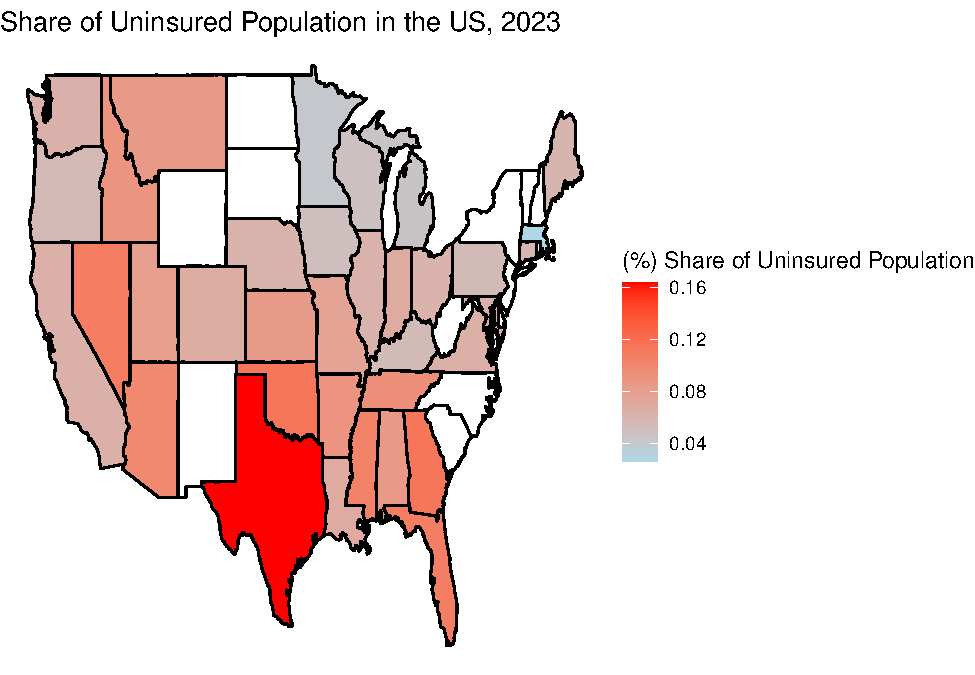
\includegraphics[width=0.85\linewidth]{template_files/figure-latex/visualize spatial-1}

\includegraphics[width=0.85\linewidth]{template_files/figure-latex/visualize spatial-2}

\textbf{Temporal Variation Visualization, Texas's Share of Uninsured
Population and Texas's GDP growth rate over time}

As we can see in the graph above, Texas emerged as a notable outlier in
our spatial variation analysis, prompting us to conduct a more
comprehensive temporal examination of the state's uninsured population
dynamics. Consequently, we analyzed Texas's proportion of uninsured
residents across a thirteen-year period from 2010 to 2023, excluding
2020 data due to potential pandemic-related anomalies. Furthermore, we
sought to investigate whether economic growth served as a contributing
factor in explaining the observed patterns in insurance coverage rates
throughout this time frame.

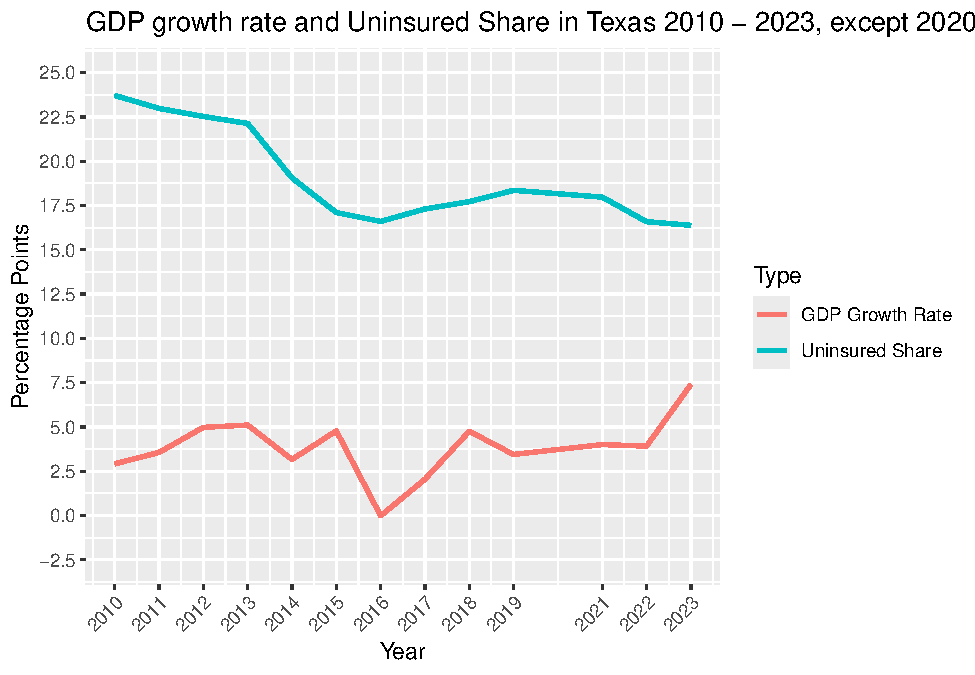
\includegraphics[width=0.8\linewidth]{template_files/figure-latex/visualization temporal-1}

\textbf{Sub-Group Variation Visualization, The Uninsured Rates of the
Middle-Income Group in 2017 in the U.S.}

Building upon findings from the Kaiser Family Foundation (2024), which
established that uninsured individuals in the United States are
disproportionately represented among low-income populations, we sought
to examine the insurance coverage status of middle-income groups who
often find themselves in a precarious position. Specifically, this
demographic typically earns insufficient income to afford private
insurance yet exceeds the eligibility thresholds for Medicaid
assistance. Moreover, we selected 2017 as our focal year, representing
the first full year following President Trump's inauguration in 2016,
thereby capturing potential early policy implications on this vulnerable
middle-income segment.

\begin{verbatim}
## [1] "First quartile (Q1): 26.625"
\end{verbatim}

\begin{verbatim}
## [1] "Second quartile (Q2): 29.35"
\end{verbatim}

\begin{verbatim}
## [1] "Third quartile (Q3): 31.25"
\end{verbatim}

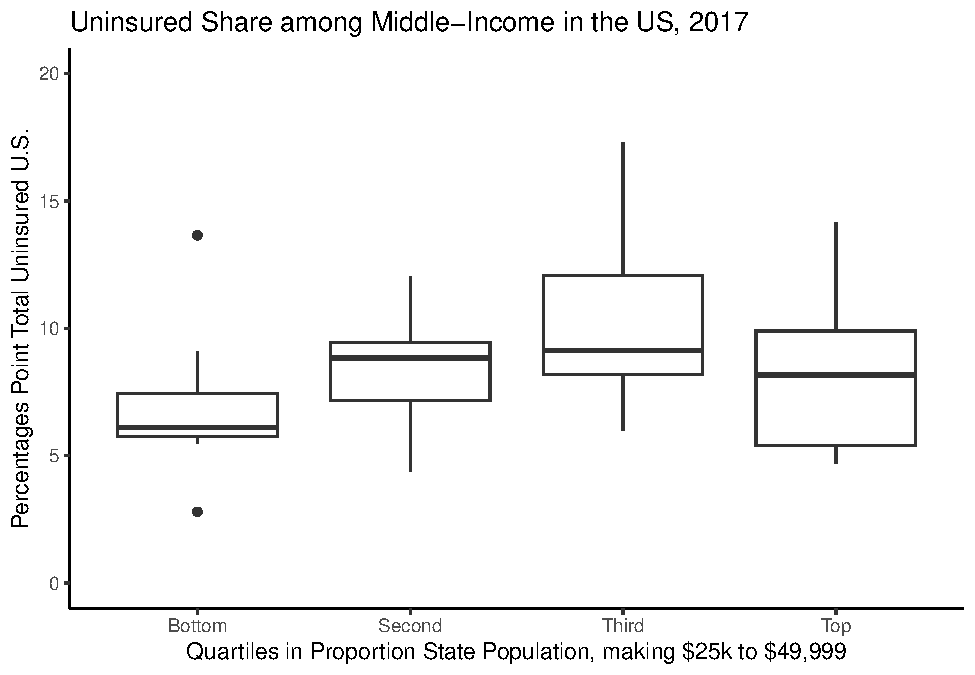
\includegraphics[width=0.8\linewidth]{template_files/figure-latex/visualization subgroup-1}

\textbf{Event Analysis Visualization, The Impact of The Implementation
of Work Requirements for Medicaid in Arkansas, 2018}

In 2018, Arkansas became the first state to implement work requirements
for Medicaid recipients as part of its Arkansas Works program, mandating
that able-bodied adults aged 19-49 demonstrate at least 80 hours of
monthly employment, education, or training activities to maintain their
Medicaid eligibility. This policy initiative was designed to encourage
workforce participation and reduce dependency on government assistance
programs. To evaluate the causal impact of this intervention, we
employed a comparative analysis framework where Arkansas serves as the
treatment group, while the remaining 43 states with available data
constitute the control group. Subsequently, we examined whether the
implementation of work requirements produced statistically significant
changes in Arkansas's uninsured rates relative to the weighted average
change observed across the control states, thereby isolating the
policy's specific effects from broader national trends in insurance
coverage.

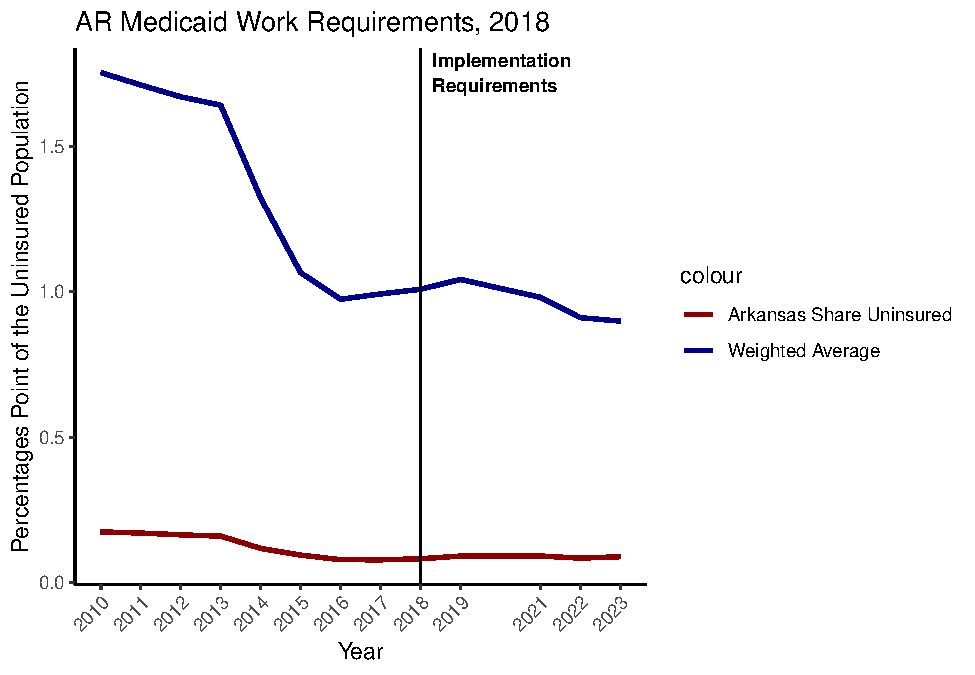
\includegraphics[width=0.8\linewidth]{template_files/figure-latex/visualization event-1}

\subsection{Identify Trends and
Patterns}\label{identify-trends-and-patterns}

\textbf{Spatial Variation Visualization, U.S. Share of The Uninsured
Population in 2023}

The spatial distribution of uninsured rates across the U.S. in 2023
reveals a pronounced regional divide. Southern states, particularly
Texas and Florida, report the highest uninsured shares. In contrast,
Northeastern and Upper Midwestern states demonstrate substantially lower
rates, likely attributable to more expansive Medicaid programs, higher
employer-based coverage, and more generous state-level health
initiatives (Bailey et al., 2017).

Western states like Nevada and Arizona present a more complex pattern,
exhibiting elevated uninsured rates despite relatively progressive
policy environments. This may reflect distinct labor market
characteristics, including higher prevalence of gig work, part-time
employment, and self-employment, which are associated with reduced
access to employer-sponsored insurance (Collins et al., 2020).

These findings support existing literature demonstrating that health
coverage in the U.S. is not solely determined by state policy, but is
fundamentally linked to employment structures, income levels, and
demographic characteristics (Davis, 2007; Sommers et al., 2012).
Consequently, even among states with similar political orientations,
uninsured rates can vary significantly based on labor market and
population dynamics.

\textbf{Temporal Variation Visualization, Texas's Share of Uninsured
Population and Texas's GDP growth rate over time}

The line graph illustrates the relationship between GDP growth rate and
uninsured share in Texas from 2010 to 2023, excluding 2020. We observe a
clear downward trend in the uninsured share, declining from
approximately 23\% to 17\% over this period. However, despite economic
fluctuations, particularly a GDP growth decline around 2016 and a spike
in between 2017 and 2018, the uninsured rate remained relatively high
and stable, especially after 2016.

This pattern suggests that economic growth alone does not ensure
increased health insurance coverage. Even during years with strong GDP
growth, Texas maintained one of the highest uninsured rates nationally.
A likely explanation is Texas's decision not to expand Medicaid under
the ACA, leaving many low-income adults without affordable coverage
options (KFF, 2023; Davis, 2007). Policy choices, rather than solely
economic performance, fundamentally shape insurance access.

\textbf{Sub-Group Variation Visualization, The Uninsured Rates of the
Middle-Income Group in 2017 in the U.S.}

The box plot displays total uninsured share per U.S. state in 2023,
grouped by quartiles of middle-income earners (those earning
\$25,000--\$49,999). The y-axis reflects overall uninsured rates, not
exclusively middle-income individuals. The second and third quartiles
demonstrate nearly identical median uninsured rates, suggesting that
higher proportions of middle-income residents do not clearly relate to
higher or lower uninsured shares.

This supports the premise that income alone does not determine insurance
coverage. Other factors including cost of living, Medicaid eligibility
requirements, and state-level policy differences play substantial roles.
Two states may have similar income distributions yet vastly different
uninsured rates due to variations in insurance affordability, healthcare
access, or Medicaid expansion status (Davis, 2007; KFF, 2023).

\textbf{Event Analysis Visualization, The Impact of The Implementation
of Work Requirements for Medicaid in Arkansas, 2018}

The graph shows uninsured share in Arkansas compared to the national
weighted average from 2010 to 2023, excluding Arkansas. Arkansas
experienced a sharp decline in uninsured rates after expanding Medicaid
under the Affordable Care Act, reaching a low around 2016--2017.
However, after implementing work requirements for Medicaid in 2018, this
trend reversed: Arkansas's uninsured rate increased while the national
average remained low and stable.

This suggests the policy negatively affected coverage. Although intended
to encourage employment, research indicates many people lost coverage
not due to unwillingness to work, but because of administrative barriers
and confusion about reporting requirements (Sommers et al., 2019).
Consequently, thousands of eligible individuals were removed from
Medicaid, increasing the uninsured share. The work requirements likely
influenced uninsured percentages by creating new obstacles to
maintaining insurance coverage, particularly for low-income adults.

\section{Part 4 -- Communicate
Findings}\label{part-4-communicate-findings}

\subsection{Summarize Key Insights}\label{summarize-key-insights}

To summarize our key insights, the spatial variation analysis
demonstrated that regional policy choices and labor market structures
significantly influence uninsured rates beyond political ideology alone.
Western states like Nevada and Arizona exhibited elevated uninsured
rates despite progressive policy environments, reflecting distinct
employment patterns including higher prevalence of gig work and
self-employment that reduce access to employer-sponsored insurance. The
temporal analysis revealed that economic growth does not automatically
translate into improved health coverage, particularly in non-expansion
states like Texas, where strong GDP growth coincided with persistently
high uninsured rates due to the absence of Medicaid expansion.

The subgroup analysis provided evidence that income distribution alone
does not fully explain variation in uninsured rates across states.
States with similar proportions of middle-income earners demonstrated
vastly different uninsured rates, indicating that factors such as cost
of living, state-specific policies, and insurance market accessibility
play substantial roles in coverage outcomes. Finally, the event analysis
of Arkansas's Medicaid work requirements illustrated how administrative
barriers can reverse coverage gains, with the policy leading to
increased uninsured rates as eligible individuals lost coverage due to
reporting difficulties and employment instability rather than
unwillingness to work. These findings collectively underscore that
achieving universal coverage requires comprehensive policy approaches
that address structural employment changes, administrative complexity,
and regional economic variations rather than relying solely on economic
growth or income-based solutions.

\subsection{Propose Solutions or Policy
Recommendations}\label{propose-solutions-or-policy-recommendations}

\textbf{Key Policy Solutions}

Based on the analysis findings, four targeted policy interventions are
recommended to address persistent uninsurance across the United States.

Enhanced federal funding should be provided to encourage remaining
non-expansion states like Texas and Florida to adopt Medicaid expansion.
The temporal analysis of Texas demonstrates that economic growth alone
cannot close coverage gaps without accompanying policy action. Despite
periods of strong GDP growth, Texas maintained one of the highest
uninsured rates nationally, suggesting that macroeconomic performance is
insufficient to guarantee insurance access. Federal incentives could
include increased matching funds or temporary enhanced federal medical
assistance percentages to make expansion financially attractive for
holdout states. This approach would address the fundamental policy gap
that leaves millions of low-income adults without affordable coverage
options.

Portable benefits systems should be developed for independent
contractors and part-time workers to address the changing nature of
employment. Western states' elevated uninsured rates reflect evolving
labor markets that traditional employer-based coverage cannot adequately
address, particularly the rise of gig work, part-time employment, and
self-employment. These workers often fall into coverage gaps, earning
too much for traditional Medicaid but lacking access to
employer-sponsored insurance. Policy solutions could include portable
benefit accounts that workers maintain across jobs, expanded association
health plans for freelancers, or modified marketplace subsidies
specifically designed for non-traditional employment arrangements.

Medicaid work requirements should be eliminated and enrollment processes
streamlined to remove administrative barriers that impede coverage
access. The Arkansas case study provides compelling evidence that work
requirements reverse coverage gains and disproportionately harm
vulnerable populations. Research indicates that many people lost
coverage not due to unwillingness to work, but because of administrative
hurdles and confusion about reporting requirements. Simplifying
enrollment procedures, reducing paperwork burdens, and eliminating
punitive work requirements would help maintain coverage continuity and
ensure that eligible individuals can access and retain benefits without
navigating unnecessarily complex bureaucratic processes.

Premium subsidies should be expanded beyond current income thresholds to
address affordability challenges that persist across income levels. The
middle-income analysis reveals that affordability problems are not
confined to the lowest income brackets, as state-level variations in
costs and policies create different financial pressures across regions.
Current subsidy structures may not adequately account for geographic
cost variations or the reality that middle-income families in high-cost
states face significant premium burdens. Expanding eligibility for
premium tax credits and cost-sharing reductions, potentially through
sliding scale adjustments based on regional cost indices, would help
address coverage gaps among moderate-income populations who currently
find insurance unaffordable despite not qualifying for existing
assistance programs.

\section{Appendix}\label{appendix}

\subsection{A.1 References}\label{a.1-references}

\begin{itemize}
\tightlist
\item
  Davis, K. (2007). \emph{Uninsured in America: Problems and possible
  solutions}. \emph{BMJ}, 334(7589), 346--348.
  \url{https://doi.org/10.1136/bmj.39091.493588.be}
\item
  KFF (2023). \emph{Key Facts About the Uninsured Population}.
  \url{https://www.kff.org/uninsured/issue-brief/key-facts-about-the-uninsured-population/}
\item
  Sommers, B. D., et al.~(2019). \emph{Medicaid Work
  Requirements---Results from the First Year in Arkansas}. \emph{New
  England Journal of Medicine}, 381(11), 1073--1082.
  \url{https://doi.org/10.1056/NEJMsr1901772}
\item
  Bailey, M. J., et al.~(2017). \emph{State Medicaid expansions and
  mortality, revisited: A cost-benefit analysis}. \emph{American Journal
  of Health Economics}, 3(4), 392--421.
  \url{https://doi.org/10.1162/AJHE_a_00080}
\item
  Collins, S. R., Gunja, M. Z., \& Aboulafia, G. N. (2020). \emph{U.S.
  health insurance coverage in 2020: A looming crisis in affordability}.
  \emph{The Commonwealth Fund}.
\item
  Sommers, B. D., Baicker, K., \& Epstein, A. M. (2012). \emph{Mortality
  and access to care among adults after state Medicaid expansions}.
  \emph{New England Journal of Medicine}, 367(11), 1025--1034.
  \url{https://doi.org/10.1056/NEJMsa1202099}
\end{itemize}

\subsection{A.2 Session Info}\label{a.2-session-info}

\url{https://github.com/catherinamikhail/Programming-for-Economists-uninsured-US-population.git}

\end{document}
